\chapter{データ実験の詳細}
\section{使用したモデルの詳細}
第三章で述べたとおり使用した対戦データは弱いAIを先番とし、強いAIを後手としている。
AIの強さは一手ごとの探索を行う時間(time)と付録Cで述べる$C_{puct}$の値によって調整した。
timeと$C_{puct}$はいずれも値が大きい程モデルは強くなると考えられる。
対戦データ生成時のパラメータは以下の表の幅からゲームごとにランダムな値を採用した。
これはパラメータの値を変化させることでゲームデータに多様性を持たせるためである。
\begin{table}[H]
	\caption{対戦データのパラメータ}
	\centering
	\scalebox{0.98}[0.98]{
		\begin{tabular}{c|c|c}
			モデル&強&弱\\ \hline
			time    & 3-5 & 0-2 \\ 
			$C_{puct}$ & 0.8-1   & 0-0.5 \\

		\end{tabular}
	}
	\label{table:battle}
\end{table}

\section{対戦結果の詳細}
2000ゲームのうち1983ゲームは強いAI(後番)の勝利となった。
また、ゲームごとの手数は75\%のゲームが36手以内で終了している。
以下にゲームの終了手数の累計グラフを示す。
\begin{figure}[t]
	\centering
	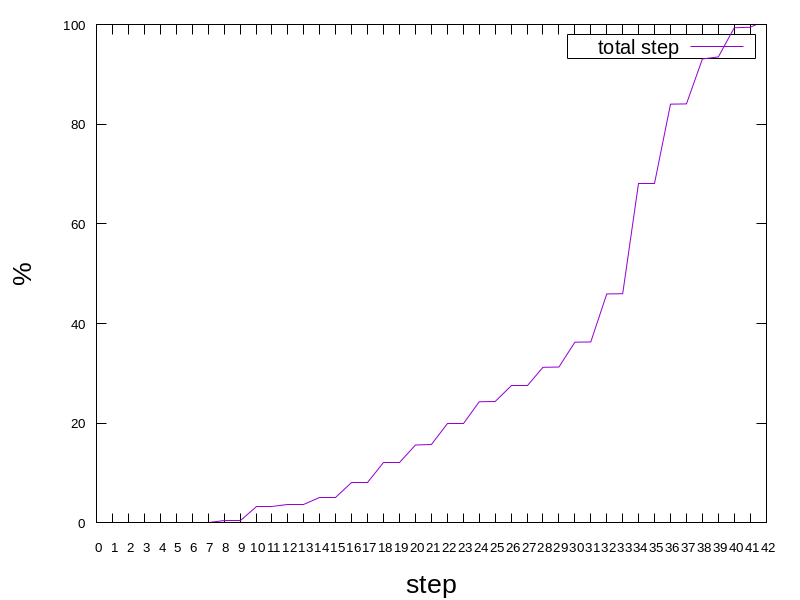
\includegraphics[width=\linewidth]{./figure/stepCum.png}
	\caption{終了手数の分布}
	\label{fig:stepCum}
\end{figure}
\section{評価指標の詳細}
本論文が提案する提案指標(group count, stone count)の計算において、盤面の座標は図\ref{fig:index}のように定められる。
\begin{figure}[t]
	\centering
	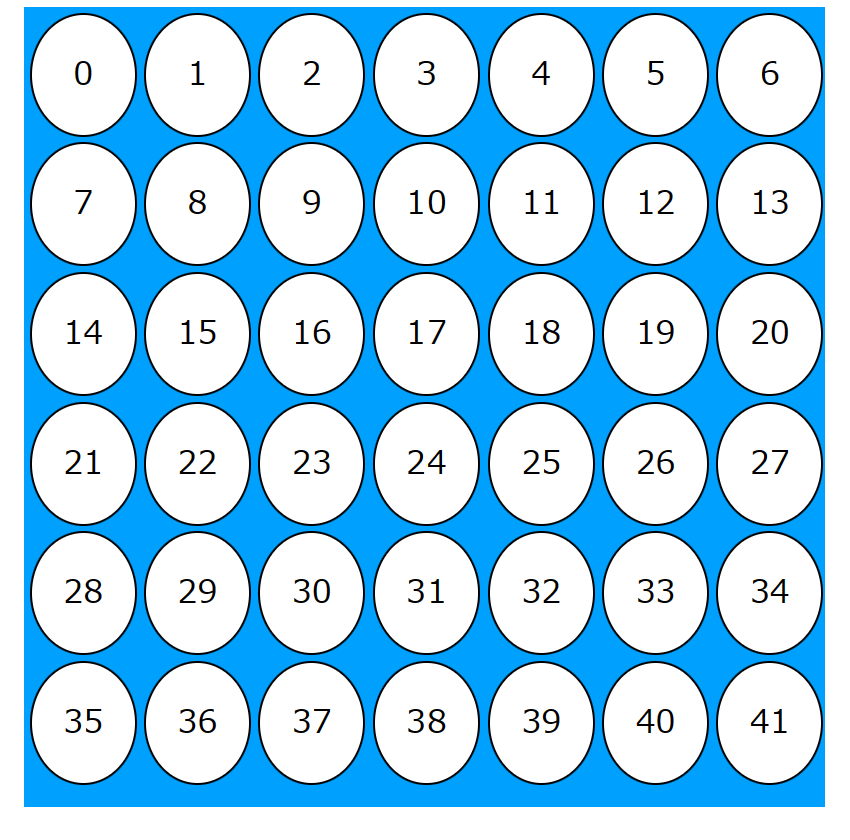
\includegraphics[width=\linewidth]{./figure/index.png}
	\caption{盤面の座標番号}
	\label{fig:index}
\end{figure}
ゲーム終了状態には以下のように4つ以上連続してつながっている石の座標$F_s$(fatal stoneの集合)とその組み合わせ$F_g$(fatal groupの集合)を記録する。
下の図の盤面は{17, 18, 19, 20, 24, 31, 38}の7つのfatal stoneと{[17, 18, 19, 20], [17, 24, 31, 38]}の二つのfatal groupを持つ
\begin{figure}[t]
	\centering
	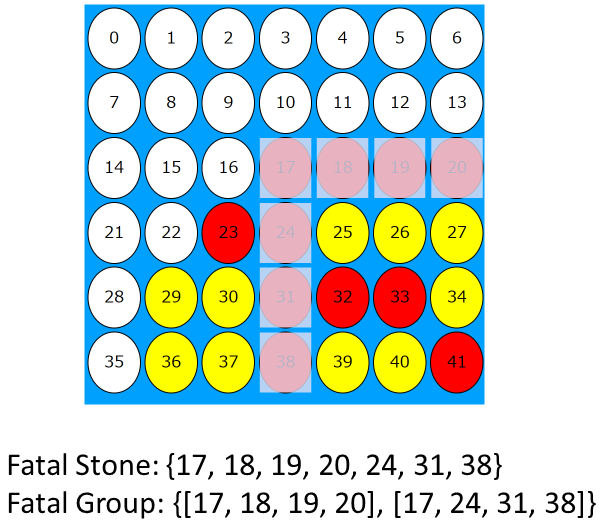
\includegraphics[width=\linewidth]{./figure/fatalGroup.png}
	\caption{fatalStoneとfatalGroup}
	\label{fig:fatalGroup}
\end{figure}
group count($C_g$), stone count($C_s$)は実際のゲームにおけるfatal groupとfatal stoneの集合(それぞれ$R_s, R_g$とする)とAIの予測によるfatal stoneとfatal groupの集合($F_g, F_s$)を比較する指標である。
どちらも値が高ければ高い程予測の精度が高いことを表す。
\subsection{group count}
fcountはfatal groupの精度を示す二値(0または1)の指標である。
\begin{equation}
	{C_g = 1 \textrm{If} F_g \cap R_g \ne \phi \textrm{Else} 0}
\end{equation}
例外として$R_g=\phi$(引き分け)の場合,$F_g$も空集合であるならばgroup countは1となる。
\subsection{stone count}
stone countはfatal stoneの精度を示す。stone countの値域は[0, 1]である。
(Count()は集合の要素数を数える関数)
\begin{equation}
	{\textrm{stone count} = \textrm{min}(\frac{\textrm{Count}(F_s \cap R_s)}{4}, 1)  }
\end{equation}
例外として$R_s=\phi$(引き分け)の場合,$F_s$も空集合であるならばstone countは1となる。
\section{データ実験における提案指標の計測}

\begin{enumerate}
	\item 比較手法: 付録?で述べた決定木の走査によりたどり着いた$F_s, F_g$によってstone count, group countを計算した
	\item 提案手法: 第三章で述べたアルゴリズムによって収集された最終状態の集合$S=\{s_{edge_1}, s_{edge_2}, ..., s_{edge_{k^l}}\}$
	    を指標ごとにグループ化する。
		\begin{itemize}
			\item group count: fatal groupによって$S$をグループ化してできた集合$\{S_{g_1}, S_{g_2}, ..., S_{g_n}\}$($S_{g_i}$は組み合わせ$g_i$がfatal groupとなっている盤面の集合)
			を要素が多い順に二つ取り出す。抽出された二つの集合$\{S_{g_{m_1}}, S_{g_{m_2}}\}$における$\{g_{m_1}, g_{m_2}\}$で構成される集合を$F_g$とし、group countを計算した。
			\item stone count: fatal stoneによって$S$をグループ化してできた集合$\{S_0, S_1, ..., S_41\}$($S_i$は番号$i$の座標がfatal stoneとなっている盤面の集合)
			を要素数が多い順に4つ取り出す。抽出された4つの集合$\{S_{m_1}, S_{m_2}, S_{m_3}, S_{m_4}\}$における$\{m_1, m_2, m_3, m_4\}$で構成される集合を$F_s$とし、stone countを計算した。
		\end{itemize}
		
\end{enumerate}

\section{データ実験に使用したモデルの詳細}
第4章に記載した表\ref{table:result-online}の結果を求める際に用いたモデルのパラメータは以下である。
\begin{table}[H]
	\caption{データ実験:使用モデルのパラメータ}
	\centering
	\scalebox{0.98}[0.98]{
		\begin{tabular}{c|c}
			パラメータ名 & 値 \\ \hline
			time    & 対戦時の後番のモデルと同じ \\ 
			$C_{puct}$    & 対戦時の後番のモデルと同じ \\
			$k$ (提案手法のみ)     & 4 \\
			$l$ (提案手法のみ)     & 2 \\
		\end{tabular}
	}
	\label{table:param-data}
\end{table}

表\ref{table:param-data}の通り、対戦データが生成された際のモデルのパラメータを使用している。
そのため本手法はモデルの構造とパラメータの値へのアクセスが可能な場合を想定したホワイトボックス的アプローチの実験であると言える。
モデルのtime, $C_{puct}$の値を固定して同様の手法を適用した場合の実験結果を次のセクションで示す。
\section{グレーボックス的手法}
モデルのパラメータを固定し、再び第四章のデータ実験を行った。パラメータの値を固定しているため、本実験はモデルの具体的なパラメータの値へのアクセスが不可能な場合にも適用可能な
グレーボックス的手法であると言える。
\begin{table}[H]
	\caption{データ実験(追加):使用モデルのパラメータ}
	\centering
	\scalebox{0.98}[0.98]{
		\begin{tabular}{c|c}
			パラメータ名 & 値 \\ \hline
			time    & 5 \\ 
			$C_{puct}$    & 1 \\
			$k$ (提案手法のみ)     & 4 \\
			$l$ (提案手法のみ)     & 2 \\
		\end{tabular}
	}
	\label{table:param-data-extra}
\end{table}

実験の結果は表\ref{table:result-offline}のようになった。第四章に記載したホワイトボックス的手法と同様に提案手法はgroup countにおいて比較手法より高い値を示した。
\begin{table}[H]
	\caption{実験結果:データ実験}
	\centering
	\scalebox{0.98}[0.98]{
		\begin{tabular}{c|c|c|c|c}
			\multicolumn{1}{c}{} & \multicolumn{2}{|c|}{group count} 
			& \multicolumn{2}{c|}{stone count}\\ \hline \hline
			手数(盤面数, 補間の有無)    & 提案手法 & 比較手法 & 提案手法 & 比較手法 \\ \hline
			19-24(9862, 無)    & \bf{0.60} & 0.44 & 0.61 & \bf{0.63} \\
			19-24(9862, 有)    & \bf{0.63} & 0.44 & 0.61 & \bf{0.63}  \\
			13-24(21022, 無)   & \bf{0.53} & 0.37 & 0.55 & \bf{0.56}  \\
			13-24(21022, 有)   & \bf{0.55} & 0.37 & 0.55 & \bf{0.56}  \\
		\end{tabular}
	}
	\label{table:result-offline}
\end{table}
